\documentclass[xetex,serif]{beamer}
\usetheme{Madrid}
 
\usepackage{xltxtra}
\usepackage[]{media9}
\XeTeXlinebreaklocale "th"
\defaultfontfeatures{Scale=1.6}
\setmainfont[
 Script=Thai,
 BoldFont={THSarabunNew Bold.ttf}, 
 ItalicFont={THSarabunNew Italic.ttf},
 BoldItalicFont={THSarabunNew BoldItalic.ttf}
 ]{THSarabunNew.ttf}
 
\title{โรคอัลไซเมอร์}
\author{กลุ่ม 1}
\date{12 มิถุนายน 2562}
\institute{ห้อง 39}
 
\begin{document}
\begin{frame}
  \maketitle
\end{frame}

\section{สาเหตุของโรคอัลไซเมอร์}

\begin{frame}{สาเหตุของโรคอัลไซเมอร์}

\begin{center}
\includemedia[
  label=some_dice,
  width=1.0\linewidth,height=0.675\linewidth, % 16:9
  addresource=video.mp4, 
  transparent,
  activate=pageopen,
  passcontext,
  flashvars={
    source=video.mp4
   &autoPlay=true % start playing on activation
   &loop=true
  }
]{}{VPlayer.swf}
% loop video
\end{center}

\end{frame}

\begin{frame}{สาเหตุของโรคอัลไซเมอร์}

  {\large \textbf{Acetylcholine}}
  \begin{itemize}
    \item เป็นสารเคมีในสมองทำหน้าที่เกี่ยวกับความจำ และกระบวนการเรียนรู้
    \item นอกจากนี้ยังเป็นสารสื่อประสาทที่ถูกหลั่งจากปลายประสาท
    \item พบได้ในสมอง ไขสันหลัง รอยเชื่อมต่อกล้ามเนื้อ รวมทั้งปมประสาทอัตโนมัติชนิดพาราซิมพาเทติก
  \end{itemize}
  \begin{center}
    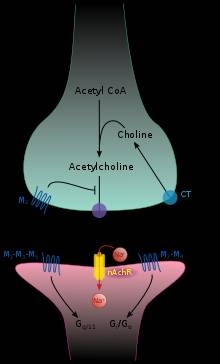
\includegraphics[height=110pt]{img0.jpg}
  \end{center}
\end{frame}

\begin{frame}{สาเหตุของโรคอัลไซเมอร์}

  {\large \textbf{Amyloid beta}}

  \begin{itemize}
    \item เกิดจากการย่อยสลายของโปรตีนขนาดใหญ่ที่เรียกว่า อะไมลอยด์พรีเคอเซอร์โปรตีน
    \item ถูกย่อยโดยเอนไซม์ที่ชื่อ เบต้าซีครีเทส ($\beta$ secretase) และแกมม่าซีครีเทส
    
    ($\gamma$ secretase)
    \item ทำให้การทำงานของสารสื่อประสาทผิดปกติไป โดยเฉพาะอย่างยิ่งทำให้สารอะเซติลโคลีนลดลง  
  \end{itemize}
  \begin{center}
    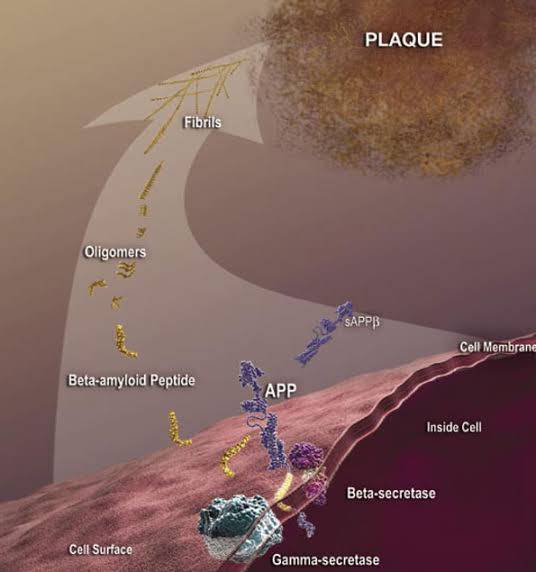
\includegraphics[height=90pt]{img1.jpg}
  \end{center}
\end{frame}

\begin{frame}{สาเหตุของโรคอัลไซเมอร์}

  {\large \textbf{Tau protein}}

  \begin{itemize}
    \item เกาะอยู่บนเส้นใยขนาดเล็กของเซลล์ประสาท
    \item ทำให้เซลล์ประสาทปกติมีความยืดหยุ่น และคงตัว *แต่ในโรคอัลไซม์เมอร์พบว่าโปรตีนเทาเกิดการเปลี่ยนแปลงทางเคมี สลายตัว และจับตัวกันเอง จนกลายเป็นก้อนและพันกันยุ่งเหยิงเรียกว่า แทงเกิ้ล หรือ นิวโรฟิบริลารี่ แทงเกิ้ล (neurofibrillary tangles, NFTs) 
  \end{itemize}
  \begin{center}
    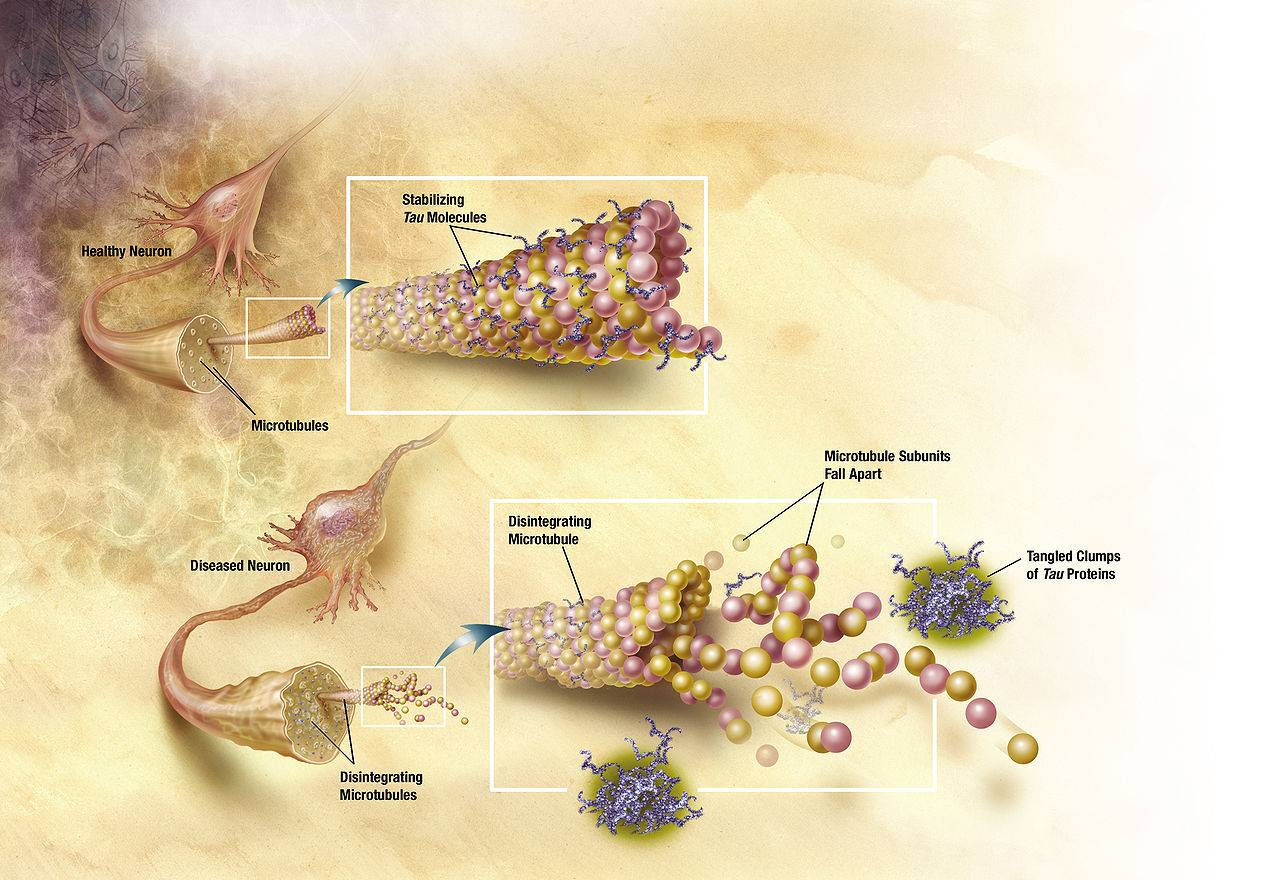
\includegraphics[height=100pt]{img2.jpg}
  \end{center}
\end{frame}

\section{ระยะอาการของโรคอัลไซเมอร์}

\begin{frame}{ระยะอาการของโรคอัลไซเมอร์}

  {\large โดยทั่วไปอาการของโรคอัลไซเมอร์จะแบ่งออกเป็น 3 ระยะหลัก ๆ ได้แก่}

  \begin{itemize}
    \item อาการระยะเริ่มแรก 
    \item อาการระยะปานกลาง 
    \item อาการระยะสุดท้าย 
  \end{itemize}
\end{frame}

\begin{frame}{ระยะอาการของโรคอัลไซเมอร์}

  {\Large \textbf{อาการระยะเริ่มแรก}}

  \begin{itemize}
    \item ลืมเกี่ยวกับบทสนทนา ชื่อสถานที่และวัตถุ 
    \item มีปัญหาในการคิดคำพูดที่ถูกต้อง 
    \item ย้ำคิดย้ำทำ 
    \item ปรับตัวได้ช้าลง และลังเลที่จะลองสิ่งใหม่ๆ 
    \item มีการเปลี่ยนแปลงทางอารมณ์ เช่น มีอาการวิตกกังวล ตื่นตระหนก สับสนเป็นระยะ ๆ
  \end{itemize}
\end{frame}

\begin{frame}{ระยะอาการของโรคอัลไซเมอร์}

  {\Large \textbf{อาการระยะปานกลาง}}

  \begin{itemize}
    \item สับสนและมึนงงมากขึ้น เช่น หลงทาง ไม่ทราบว่าตอนนี้เวลาเท่าไหร่ หรือวันอะไร 
    \item เกิดอาการหลงผิด (เชื่อสิ่งที่ไม่จริง)  หรือรู้สึกหวาดระแวงและสงสัยในผู้ดูแลหรือแม้แต่สมาชิกในครอบครัว 
    \item มีปัญหาเกี่ยวกับการพูดหรือภาษา (aphasia) 
    \item นอนหลับไม่เต็มที่ 
    \item เกิดการเปลี่ยนแปลงอารมณ์มากขึ้น 
    \item เกิดภาพหลอน 
    \item เป็นเรื่องยากที่จะจำชื่อคนที่พวกเขารู้จัก 
    \item มักต้องการการสนับสนุนเพื่อช่วยเหลือในชีวิตประจำวัน
  \end{itemize}
\end{frame}

\begin{frame}{ระยะอาการของโรคอัลไซเมอร์}

  {\Large \textbf{อาการระยะสุดท้าย}}

  \begin{itemize}
    \item เคี้ยวอาหารและกลืนได้ลำบาก (dysphagia)
    \item ยากที่จะเคลื่อนที่หรือเดินไปรอบ ๆ โดยไม่ได้รับความช่วยเหลือ
    \item น้ำหนักตัวลดลงอย่างหนัก
    \item เกิดภาวะปัสสาวะหรืออุจจาระเล็ด
    \item สูญเสียความสามารถในการสื่อสารมากขึ้นเรื่อย ๆ
    \item เกิดปัญหาสำคัญของทั้งความจำระยะสั้นและความจำระยะยาว
    \item อาจก้าวร้าว เรียกร้องความสนใจ และระแวงคนรอบข้าง
    \item อาจต้องได้รับการดูแลตลอดเวลา
  \end{itemize}
\end{frame}

\section{แนวทางการป้องกันโรคอัลไซเมอร์}

\begin{frame}{แนวทางการป้องกันโรคอัลไซเมอร์}
  \begin{itemize}
    \item การออกกําลังกายอย่างสมําเสมอ อย่างน้อยวันละ 150 นาที (Regular exercise) 
    \item การฝึกการเข้าร่วมสังคม (Social Engagement) เช่น การทําจิตอาสา ท่องเที่ยว หรือ หาเพื่อนใหม่ในวัยที่ใกล้เคียงกัน
    \item  การกินอาหารอย่างมีประสิทธิภาพ (Healthy Diet)  โดยรับประทานอาหารที่มี Omega 3 ในปริมาณที่สูง และครบ 5 หมู่ ตลอดทุกมื้อ ทั้งนี้มีอาหารเเบบนึงที่ได้ถูกเเนะนําโดยองค์กรเกษตรของสหรัฐ (USDA)
  \end{itemize}
\end{frame}

\begin{frame}{แนวทางการป้องกันโรคอัลไซเมอร์}
  \begin{itemize}
    \item อาหารเเบบ Mediterranean Diet ซึ่งเน้นการกิน ผัก ธัญพืช เเละ หลีกเลี่ยงสัตว์เนื้อเเดง มาทาน อาหารทะเลเเทน
  \end{itemize}
  \begin{center}
    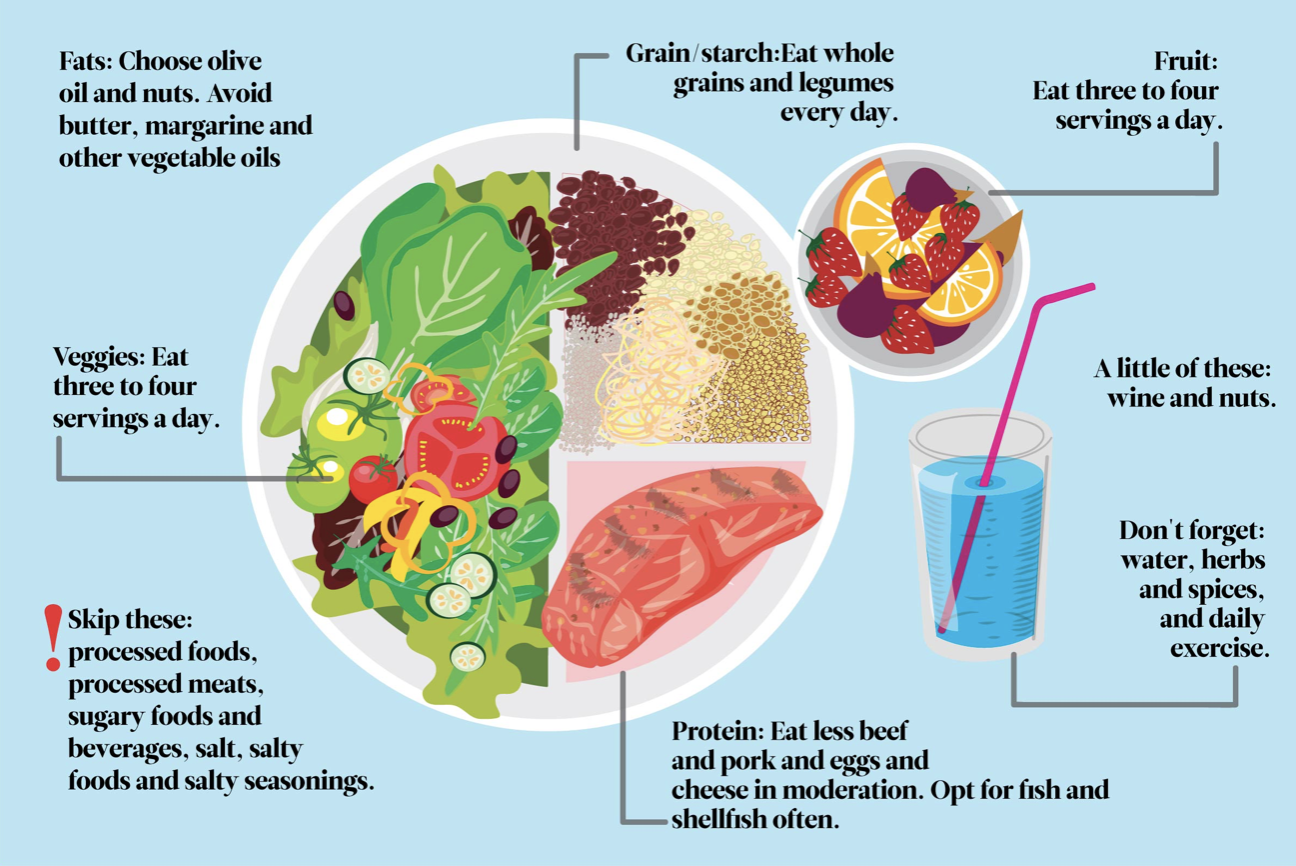
\includegraphics[width=200pt]{img3.png}
  \end{center}

\end{frame}

\begin{frame}{แนวทางการป้องกันโรคอัลไซเมอร์}
  \begin{itemize}
    \item การบำบัดอย่างถูกวิธี (Mental Stimulation) โดย ฝึกเล่นเกมส์ลับสมองประลองปัญหา หรือ ฝึกจําชื่อคนรอบข้าง
    \item การนอนหลับอย่างมีประสิทธิภาพ (Quality sleep) หลับเป็นเวลาอย่างน้อย 8 ชั่วโมงเต็ม
    \item หลีกเลี่ยง การสูบบุหรี่ หรือ เครื่องดื่มแอลกอฮอล์ ให้มากที่สุด
  \end{itemize}
\end{frame}

\section{ปัจจัยเสี่ยง}

\begin{frame}{ปัจจัยเสี่ยง}
  \begin{itemize}
    \item อายุ
    \item พันธุกรรม
    \item กลุ่มอาการดาวน์
    \item ผู้ที่เคยได้รับบาดเจ็บที่ศีรษะอย่างรุนแรง
    \item โรคหลอดเลือดหัวใจ
  \end{itemize}
\end{frame}

\end{document}